\documentclass[10pt,a4paper]{article}
\usepackage[utf8]{inputenc}
\usepackage{amsmath}
\usepackage{amsfonts}
\usepackage{amssymb}
\usepackage{makeidx}
\usepackage{graphicx}
\usepackage{framed, color}
\usepackage{colortbl}
\usepackage{multicol}
\usepackage{fullpage}
\usepackage{float}
\usepackage{array}
\usepackage{pgf}
\usepackage{pgfpages}

\pgfpagesdeclarelayout{boxed}
{
  \edef\pgfpageoptionborder{0pt}
}
{
  \pgfpagesphysicalpageoptions
  {%
    logical pages=1,%
  }
  \pgfpageslogicalpageoptions{1}
  {
    border code=\pgfsetlinewidth{2pt}\pgfstroke,%
%    border shrink=\pgfpageoptionborder,%
    resized width=.9\pgfphysicalwidth,%
    resized height=.9\pgfphysicalheight,%
    center=\pgfpoint{.5\pgfphysicalwidth}{.5\pgfphysicalheight}%
  }%
}

\pgfpagesuselayout{boxed}

\definecolor{boxcolour}{rgb}{0.0, 0.0, 0.0}
\definecolor{textcolour}{rgb}{1.0, 1.0, 0.0}

\begin{document}
\begin{center}
	\colorbox[rgb]{0.0, 0.0, 0.0}
	{
	\begin{minipage}[c][3em][c]{\textwidth}
		{\color{textcolour}
			{
			\begin{Large}
				\textbf{ROBOT SPECIFICATION}
			\end{Large}
			}
		}
	\end{minipage}
	}
\end{center}

\begin{multicols}{2}
\begin{table}[H]
	\begin{tabular}{|m{5.7cm}|m{1.15cm}|}
		\hline
		\rowcolor[rgb]{0.0, 0.0, 0.0}
		{\color{textcolour}\textbf{{PHYSICAL SPECIFICATIONS}}} & \\
		\hline
		Height (cm) & 45.5 \\
		\hline
		Weight (kg) & 2.9 \\
		\hline
		Walking Speed (cm/s) & 15 \\
		\hline
	\end{tabular}
\end{table}

\begin{table}[H]
	\begin{tabular}{|m{5.7cm}|m{1.15cm}|}
		\hline
		\rowcolor[rgb]{0.0, 0.0, 0.0}
		{\color{textcolour}\textbf{{DEGREES OF FREEDOM}}} & \\
		\hline
		Legs (each) & 6 \\
		\hline
		Arms (each) & 3 \\
		\hline
		Neck & 2 \\
		\hline
		& \\
		\hline
		\textbf{Total} & \textbf{20} \\
		\hline
	\end{tabular}
\end{table}

\begin{table}[H]
	\begin{tabular}{|m{5.7cm}|m{1.15cm}|}
		\hline
		\rowcolor[rgb]{0.0, 0.0, 0.0}
		{\color{textcolour}\textbf{{MOTORS AND SENSORS}}} & \\
		\hline
		Dynamixel MX-28 Servo & x20 \\
		\hline
		C905 USB 2MP Camera w/ Mic. & x1 \\
		\hline
		Additional Microphone & x1 \\
		\hline
		3-axis Gyroscope & x1 \\
		\hline
		3-axis Accelerometer & x1 \\
		\hline
	\end{tabular}
\end{table}

\begin{table}[H]
	\begin{tabular}{|m{5.75cm}|m{1.15cm}|}
		\hline
		\rowcolor[rgb]{0.0, 0.0, 0.0}
		{\color{textcolour}\textbf{{COMPUTING UNITS}}} & \\
		\hline
		Intel Atom ZS30 & 1.66GHz \\
		\hline
		CM730 Management Controller & 72MHz \\
		\hline
	\end{tabular}
\end{table}

\columnbreak

\begin{center}
	\colorbox[rgb]{0.0, 0.0, 0.0}
	{
	\begin{minipage}[c][3.5em][c]{0.45\textwidth}
		\begin{center}
			{\color{textcolour}
				{
				\textbf{THE UNIVERSITY OF NEWCASTLE \\
				(AUSTRALIA)}
				}
			}
		\end{center}
	\end{minipage}
	}
\end{center}

\begin{figure}[H]
	\begin{center}
		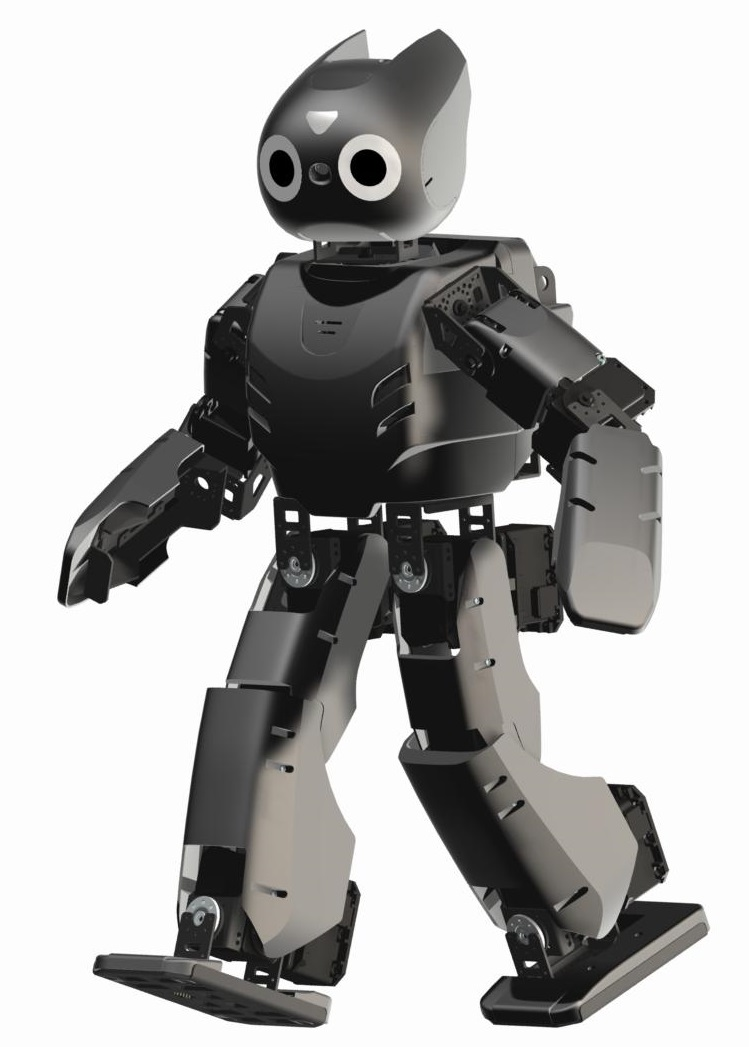
\includegraphics[scale=0.3]{darwin.png}\\
		\textbf{DARwIn-OP Robot}.
	\end{center}
\end{figure}

\end{multicols}

\begin{center}
	
\includegraphics[scale=0.8]{nubots_logo.png}
\end{center}

\end{document}